\documentclass[11pt, oneside]{article} 
\usepackage{geometry}
\geometry{letterpaper} 
\usepackage{graphicx}
	
\usepackage{amssymb}
\usepackage{amsmath}
\usepackage{parskip}
\usepackage{color}
\usepackage{hyperref}

\graphicspath{{/Users/telliott_admin/Tex/png/}}
% \begin{center} 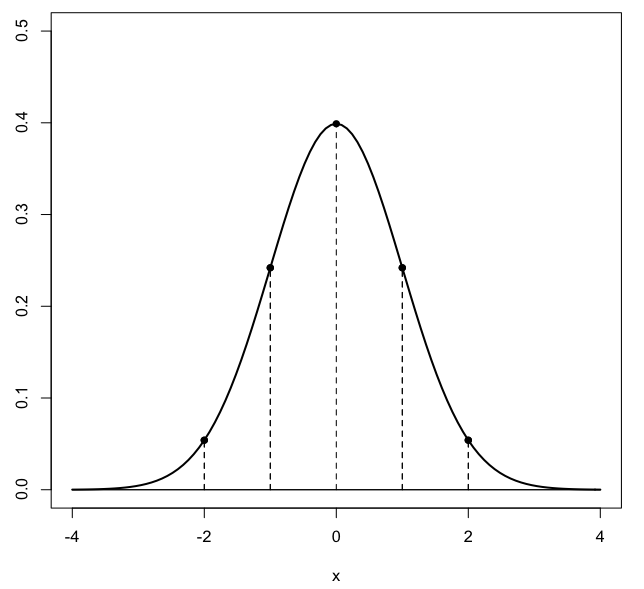
\includegraphics [scale=0.4] {gauss3.png} \end{center}

\title{Attraction of the earth}
\date{}

\begin{document}
\maketitle
\Large

\label{sec:Newton_point_mass}

Here we derive what is probably Newton's most famous result, that the mass of a spherical body behaves in terms of gravitational attraction as if it were concentrated as a "point mass" at the very center of the sphere.
\begin{center} 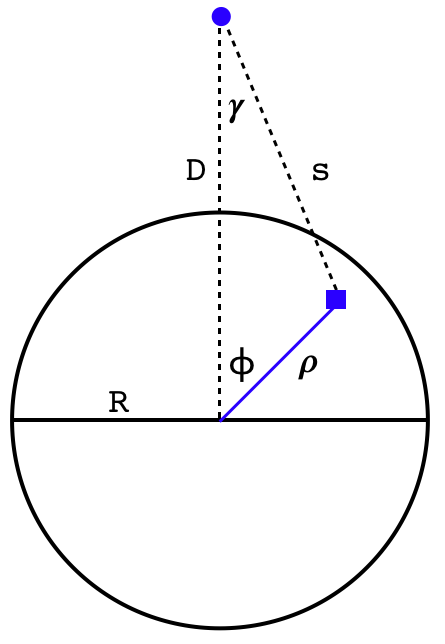
\includegraphics [scale=0.35] {newton_volume.png} \end{center}
Our notation is shown in the figure.  A point mass $m$ (blue circle) lies at a distance $D$ from the sphere's center.  Strang and Kline both use $D$ for this, so I have retained it.  The sphere has mass $M$ and radius $R$.

For the ray from the center to the volume element (or a part of a spherical belt, see later) I have used $\rho$ from Strang, while $s$ is the distance from the volume element to the test mass $m$.  

We are free to choose a coordinate system;  it is convenient to orient the $z$-axis so that it aligns with $D$;  the ray of distance $\rho$ to the little volume element $dV$ (blue square) makes the usual polar angle $\phi$ as shown.  We will also need the angle $\gamma$.
\begin{center} 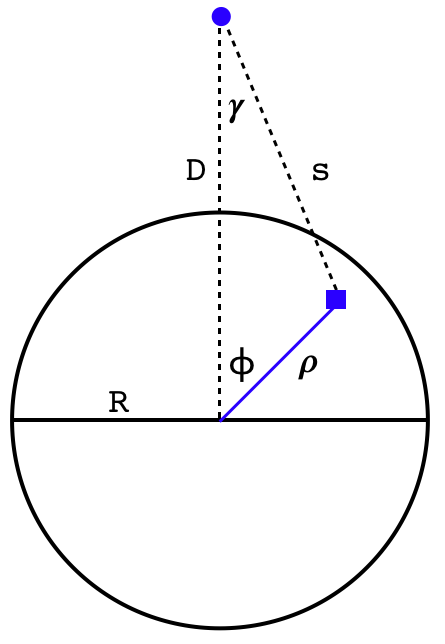
\includegraphics [scale=0.3] {newton_volume.png} \end{center}
There are two different ways of proceeding.  One, as indicated by use of $dV$, is to do a triple integral over the volume.  Spherical coordinates are best for this, as always.  For this approach, we integrate first over $\phi$, then over $\rho$ and finally add $2 \pi$ from the radial angle $\theta$, which is the outer integral.

An alternative approach is to consider a hollow shell, with $\rho$ fixed.  One first proves that the shell acts as if its mass were at the center, then many layers of concentric shells all add up to the total result.  The shell approach is not really that much different from the volume integral, which is relatively simple to do in the order given above, once we massage it a bit.

There is another fairly distinct variation for both methods, which I learned from Kline, and that is to use $s$ rather than $\phi$ as the variable of integration.  I had never thought of doing that!  

Using $s$ as the variable combined with the method of shells gives an easy extension to a result that we have already used in the book, for the problem with a \hyperlink{Earth_tunnel}{\textbf{tunnel}}
 through the earth.  We cover that in the next chapter.

\subsection*{setting up the integral}

The inverse square law for gravitation says that the force varies like $1/s^2$ for each small mass element $dM$ contained in a small volume element $dV$.

The force on the test mass $m$ due to each little piece of mass is
\[ dF = \frac{Gm}{s^2} \ dM \]
where $dM = M/V \ dV$
so
\[ dF = \frac{GmM}{V} \ \frac{1} {s^2} \ dV \]
Thus, we will have a constant factor of $GmM/V$ multiplying the result.  We do not write this any more but remember it for later.

In addition to the fact that the distance $s$ is a variable, the interesting aspect of the integral is that the force, which acts in the direction of $s$, has a sideways component with respect to $D$, namely $F \sin \gamma$, that cancels by radial symmetry, and a vertical component $F \cos \gamma$, which does not cancel.

Thus, to get the part of the force that we care about, the part that does not cancel, we have our remembered constant times the summed contributions from each little piece of volume $dV$:
\[ \int_V \frac{1}{s^2} \cos \gamma \ dV \]
\[ = \iiint  \ [ \frac{1}{s^2} \cos \gamma \ ] \ \rho^2 \sin \phi \ d \rho \ d \phi \ d \theta \]

It turns out that these two effects (of $1/s^2$ and $\cos \gamma$) even out so that the value of the integral turns out to be $1/D^2$ times the volume.  We talked about the average value of a function \hyperref[sec:Average_value]{\textbf{here}}.  We say that the average value of the function
\[ [ \frac{1}{s^2} \cos \gamma \ ] \] 
is $1/D^2$.

\subsection*{integral using $\phi$}
The inner integral is taken with respect to $\phi$ (holding $\rho$ and $\theta$ constant).  
\[ I = \int  \ [ \frac{1}{s^2} \cos \gamma \ ] \ \rho^2 \sin \phi \ d \phi  \]
We come up against the complication that $s$ and $\gamma$ are themselves both variables.  To make progress, we must express everything in terms of the single variable, $\phi$.
\begin{center} 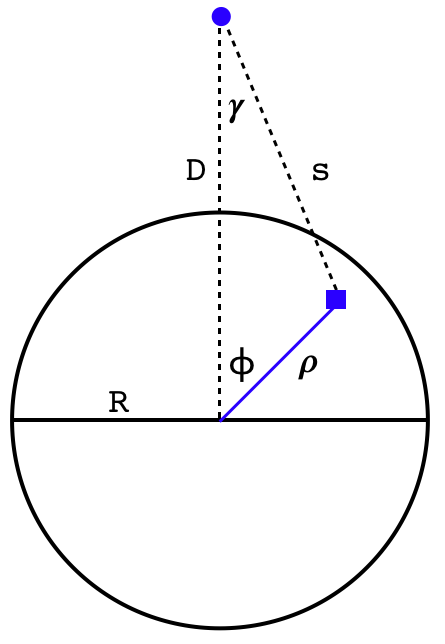
\includegraphics [scale=0.3] {newton_volume.png} \end{center}

The law of cosines comes to the rescue.  First, to get $s^2$ in terms of $\phi$
\[ s^2 = D^2 + \rho^2 - 2 D \rho \cos \phi \]
And then for $\gamma$:
\[ \rho^2 = D^2 + s^2 - 2Ds \cos \gamma \]
\[ \cos \gamma = \frac{D^2 + s^2 - \rho^2}{2Ds} \]
For simplicity, we substitute only for $\cos \gamma$ and not yet for $s^2$ 
\[ I = \int \frac{1}{s^2} \ [ \  \frac{D^2 + s^2 - \rho^2}{2Ds}  \ ] \ \rho^2 \sin \phi \ d \phi \]
Even after showing that restraint, I think we can agree that this looks like a bit of a mess.  

But now we have an inspiration! Make the substitution:
\[ u = s^2 \]
\[ = D^2 + \rho^2 - 2 D \rho \cos \phi \]
The derivative is
\[ du = 2 D \rho \ \sin \phi \ d \phi \]
\[ \rho \ \sin \phi \ d \phi = \frac{1}{2D} \ du \]

With that substitution we generate a factor of $\sin \phi \ d \phi$ in terms of something related to $s^2$ and can see a path forward:
\[ I = \int \frac{1}{s^2} \ [ \  \frac{D^2 + s^2 - \rho^2}{2Ds}  \ ] \ \rho^2 \sin \phi \ d \phi \]
\[ = \int \frac{1}{u} \cdot \frac{u + D^2 - \rho^2}{2D \sqrt{u}} \cdot \rho \cdot \frac{1}{2D} \ du\]
\[ = \frac{\rho}{4D^2} \int \frac{u + D^2 - \rho^2}{u^{3/2}} \ du \]
The integral breaks into two parts which are pretty easy
\[  = \frac{\rho}{4D^2} \ [ \  \int \frac{1}{\sqrt{u}} \ du + \int \frac{D^2 - \rho^2}{u^{3/2}} \ du \ ]  \]
\[ = \frac{\rho}{4D^2} \ [ \ 2 \sqrt{u} - 2 \ \frac{D^2 - \rho^2}{\sqrt{u}}  \ ] \]
\[ = \frac{\rho}{2D^2} \ [ \ \sqrt{u} - \ \frac{D^2 - \rho^2}{\sqrt{u}}  \ ] \]

Now, reverse the substitution, but do it gradually.  Think about
\[ u = s^2 = D^2 + \rho^2 - 2 D \rho \cos \phi \]
The bounds on $\phi$ are the usual $[0,\pi]$  At the upper bound $\cos \phi = -1$ and
\[ u = D^2 + \rho^2 + 2 D \rho = (D + \rho)^2 \]
\[ \sqrt{u} = D + \rho \]
So the term in brackets is 
\[ \sqrt{u} - \ \frac{D^2 - \rho^2}{\sqrt{u}} \]
\[ = D + \rho - \frac{(D + \rho)(D - \rho)}{D + \rho} = 2 \rho \]
You don't see that kind of simplification every day!

At the lower bound, $\cos \phi = 1$ and
\[ u = D^2 + \rho^2 - 2 D \rho = (D - \rho)^2 \]
\[ \sqrt{u} = D - \rho \]
The term in brackets is
\[ = D - \rho - \frac{(D + \rho)(D - \rho)}{D - \rho} = - 2 \rho \]
Since we subtract the value at the lower bound, we get another minus sign and the terms in the brackets add up to $4 \rho$.  The whole integral is
\[ I = \frac{\rho}{2D^2} \cdot 4 \rho = 2 \frac{\rho^2}{D^2} \]

To finish up, integrate next over $\rho$ and obtain
\[ \frac{2}{D^2} \int_0^R \rho^2 \ d \rho = \frac{2}{D^2} \ \frac{R^3}{3} \]
Finally, we pick up $2 \pi$ from the outer integral:
\[ \frac{4}{3} \pi R^3 \ \frac{1}{D^2} = \frac{V}{D^2}  \]

Recall that we left aside a constant factor of $mMG$ divided by the volume $V$.  Hence the force is:
\[ F = \frac{mMG}{V} \ \frac{V}{D^2} = \frac{mMG}{D^2}  \]

The essence of our result is that
\[ \int_V \ [ \ \frac{1}{s^2} \cos \gamma \ ] \ dV = \frac{V}{D^2}  \]
The \emph{average value} of $f(x,y,z)$ is defined to be
\[ \frac{\int_V f(x,y,z) \ dV}{\int_V \ dV} \]

The average value of the function $1/s^2 \ \cos \gamma$ taken over the whole sphere is $V/D^2$ divided by $V$ or just $1/D^2$.  
\begin{center} 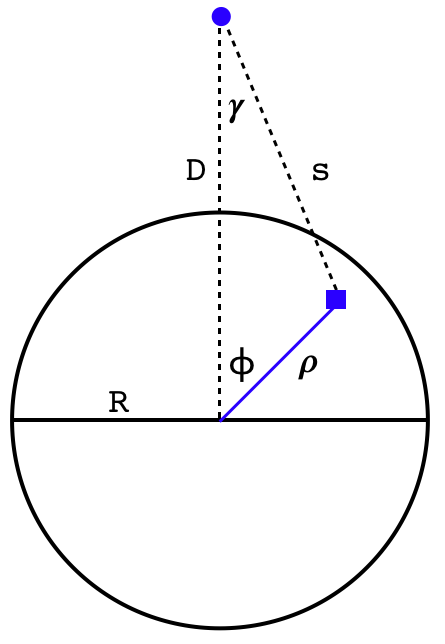
\includegraphics [scale=0.35] {newton_volume.png} \end{center}
Remarkable.

\end{document}